\newpage{}
\section{Problema A: Armando el polígono}
\textbf{Peso del ejercicio: 10}

\subsection{Descripción del Problema}

Originalmente se tiene una triangulación válida de un polígono (no necesariamente convexo) de $N$ vértices  y se desea recuperar el polígono original. La triangulación viene dada por $N-2$ triángulos, donde para cada triángulo se dan los $3$ vértices del polígono que lo conforman.

\subsection{Resolución del Problema}

Dado un polígono, lo primero que vamos a hacer es intentar diferenciar entre los segmentos que definen al polígono (que de ahora en adelante llamaremos \textbf{externos}), y a los segmentos que solo son parte de la triangulación (que de ahora en adelante llamaremos \textbf{internos}). Para mayor claridad, obsérvese la siguiente figura donde los segmentos \textit{externos} se encuentran marcados con mayor grosor.

\begin{center}
	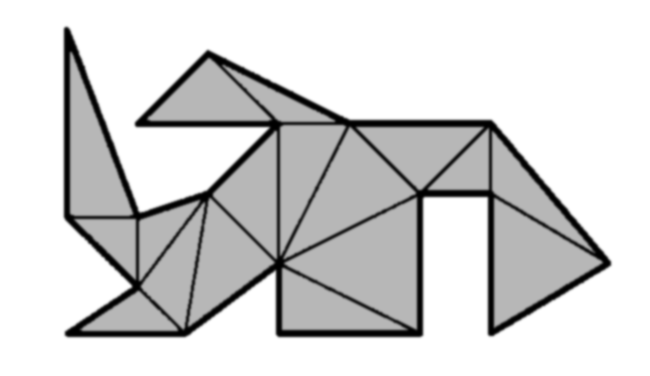
\includegraphics[scale=0.2]{triangulacion.png}
\end{center}

Para poder diferenciarlos, debemos encontrar una propiedad que podamos chequear y que solo cumplan los segmentos \textbf{externos}.
\begin{itemize}
	\item \textbf{Observación 1}: Todo segmento de la triangulación separa a dos regiones (donde consideramos al plano exterior al polígono como región). Notar que no hace falta considerar casos donde un segmento toca dos veces a la misma región porque no hay triángulos degenerados (ninguna arista es puente en el grafo planar dado por la triangulación)
	\item \textbf{Observación 2}: Si llamamos $\mathcal{T}$ a la triangulacicón y consideramos $\mathcal{V}(T)$ para $T \in \mathcal{T}$ como el conjunto de vértices del triángulo $T$. Entonces $\mathcal{V} = \bigcup\limits_{T \in \mathcal{T}} \mathcal{V}(T)$, donde $\mathcal{V}$ representa el conjunto de vértices del polígono.
\end{itemize}

Usando la Observación 1, basta notar que si iteramos por los triángulos, aquellos segmentos que aparecen en solamente un triángulo son los que llamamos \textbf{externos} y delimitan el polígono.

Una vez que tenemos identificados estos segmentos, resta identificar al vértice de menor coordenada x (desempatando por coordenada y), para luego dictar a los vértices en sentido horario. A este orden entre puntos (menor coordenada x desempatando por y) lo vamos a notar por "$\sqsubseteq$"

Para esta última parte, como ya tenemos los segmentos del polígono, podemos guardarnos para cada vértice sus dos vecinos. Luego, otenemos el mímnimo de los puntos (en el orden dado por $\sqsubseteq$), que llamaremos $v$. 

De los dos vecinos de $v$ queremos el que sigue en sentido horario, como $v$ es el de menor coordenada $"x"$ (desempatando por $"y"$), de sus dos vecinos el que sigue en sentido horario es el de mayor coordenada $y$ (pensar a los dos vectores que salen de $v$ normalizados y situarlos al borde de la circunferencia unitaria centrada en $v$). A partir de ese momento, simplemente debemos seguir moviéndonos al vecino no visitado del vértice en cuestión (recordar que cada vértice tiene exactamente dos vecinos en el polígono).

\subsection{Algoritmo y Análisis de Complejidad}

\begin{enumerate}
	\item Leemos y creamos un árbol binario de búsqueda auto-balanceado,que llamaremos $\mathcal{B}_1$ solo por simplicidad. Donde cada nodo representará a un segmento y guardará un contador por nodo que indique cuántos triángulos lo utilizan (Notar que esto equivale a utilizar un \texttt{map} en \texttt{C++}). $\mathcal{O}(1)$
	
	\item Al leer la entrada, por cada triángulo, consideramos los 3 segmentos que define, y aumentamos en $1$ al contador del nodo en $\mathcal{B}_1$ que representa a cada segmento.  $\mathcal{O}(3(N-2) \text{log}(N-2)) = \mathcal{O}(N \text{log}(N))$, donde nos basamos en la complejidad de $\texttt{map}$ para la inserción/búsqueda que es la dada por un "red-black-tree" (logarítmica en el tamaño).
	\item Creamos otro árbol binario de búsqueda auto-balanceado donde cada nodo representará a un punto del polígono, y guardará a su vez un conjunto con sus dos vecinos (exactamente 2). A este árbol lo vamos a llamar $\mathcal{B}_2$. $\mathcal{O}(1)$
	\item Iteramos por los segmentos en $\mathcal{B}_1$ y para cada segmento que aparezca en un solo triángulo (el contador es igual a 1), agregamos en $\mathcal{B}_2$ a ambos extremos del segmento, y agregamos que ambos son vecinos entre sí, agregando a ambos en sus conjuntos de vecinos. $\mathcal{O}(3(N-2)\text{log}(3(N-2)))$
	\item Obtenemos al menor de los vértices en $\mathcal{B}_2$, usando el orden dado por "$\sqsubseteq$". $\mathcal{O}(N)$ si iteramos en todos los nodos, $\mathcal{O}(1)$ si $\mathcal{B}_2$ está ordenado según $\sqsubseteq$.
	\item Imprimimos el vértice obtenido en 5 y calculamos al siguiente vértice en sentido horario (o sea, de sus dos vecinos, chequear el que tiene mayor coordenada "y"). $\mathcal{O}(1)$.
	\item Repetimos $N-1$ veces (por vértice restante)  el siguiente procedimiento:
	\begin{enumerate}
		\item Imprimimos el vértice actual. $\mathcal{O}(1)$
		\item Calculamos al vértice que le sigue al actual como el vecino de él que es distinto al anteriormente visitado. $\mathcal{O}(1)$
		\item actualizamos al anterior y al actual.$\mathcal{O}(1)$
	\end{enumerate}
	Entonces esta parte nos queda $\mathcal{O}(N)$
\end{enumerate}

Sumando bajo la notación de $\mathcal{O}$ nos queda que la complejidad total del algoritmo es $\mathcal{O}(N\text{log}(N))$



\subsection{Detalles de implementación}

Para una correcta implementación, es importante tener en cuenta cómo representamos a los segmentos, para ello vamos a tomar la convención de que un segmento $S = [P_1, P_2]$ cumple que $P_1 \sqsubseteq P_2$. De esta forma, dados dos puntos distintos tenemos una única representación para un segmento.

Otro detalle a tener en cuenta es que la complejidad total puede mejorarse si se utiliza \textit{hashing}, léase \texttt{unordered} \_ \texttt{map}. Pues a la hora de tener un contador para cada segmento, no nos interesa su orden. Análogamente para los puntos del polígono y sus dos vecinos, que se usan para dictar los vértices en orden horario.
 En este caso, obtenemos una complejidad de $\mathcal{O}(N)$ si se implementa correctamente (y la función de hashing es suficientemente buena).  


\newpage
\subsection{Código de la solución}
\lstset{inputencoding=utf8/latin1}
\lstinputlisting[numbers = left]{../src/ej1/ej1.cpp}

